\hypertarget{protocol_t_p_chart_data_scaling-p}{
\section{$<$ TPChartDataScaling $>$ Protocol Reference}
\label{protocol_t_p_chart_data_scaling-p}\index{TPChartDataScaling-p@{TPChartDataScaling-p}}
}
{\tt \#import $<$TPParameterProtocols.h$>$}

Inheritance diagram for $<$ TPChartDataScaling $>$::\begin{figure}[H]
\begin{center}
\leavevmode
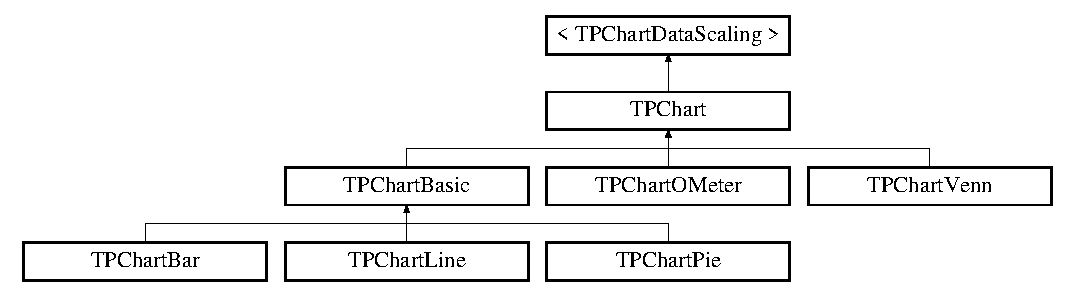
\includegraphics[height=3.5443cm]{protocol_t_p_chart_data_scaling-p}
\end{center}
\end{figure}
\subsection*{Public Member Functions}
\begin{CompactItemize}
\item 
(void) - \hyperlink{protocol_t_p_chart_data_scaling-p_940844c4e44e6f253f1b9b389646793d}{setScalingData:}
\end{CompactItemize}


\subsection{Detailed Description}
Protocol for charts who have data scaling 

\subsection{Member Function Documentation}
\hypertarget{protocol_t_p_chart_data_scaling-p_940844c4e44e6f253f1b9b389646793d}{
\index{TPChartDataScaling-p@{TPChartDataScaling-p}!setScalingData:@{setScalingData:}}
\index{setScalingData:@{setScalingData:}!TPChartDataScaling-p@{TPChartDataScaling-p}}
\subsubsection[{setScalingData:}]{\setlength{\rightskip}{0pt plus 5cm}- (void) setScalingData: ({\bf TPParameterDataScaling} $\ast$) {\em scalingData}}}
\label{protocol_t_p_chart_data_scaling-p_940844c4e44e6f253f1b9b389646793d}


\begin{Desc}
\item[Parameters:]
\begin{description}
\item[{\em scalingData}]scaling data \end{description}
\end{Desc}


The documentation for this protocol was generated from the following file:\begin{CompactItemize}
\item 
TPParameterProtocols.h\end{CompactItemize}
